% !TEX program = pdflatex
% Tufte-style manual for Hessian-based filters and neuriteness

\documentclass[a4paper,justified]{tufte-book}

\usepackage{amsmath,amssymb}
\usepackage{graphicx}
\usepackage{booktabs}
\usepackage{hyperref}
\usepackage{listings}
\usepackage{xcolor}
\usepackage{tikz}
\usetikzlibrary{arrows.meta, positioning}


\definecolor{codegray}{rgb}{0.95,0.95,0.95}
\lstset{
	backgroundcolor=\color{codegray},
	basicstyle=\ttfamily\small,
	frame=single,
	breaklines=true,
	columns=fullflexible
}

\title{Hessian-Based Image Filters}
\author{ }
\date{ }

\begin{document}
	\maketitle
	

	\tableofcontents
	
	\newpage
	
	% -----------------------------------------------------------------------------
	\section{Summary}
	
	This manual documents a modular MATLAB package for Hessian-based image filtering, including multiscale detectors such as vesselness and ridge filters, and a faithful implementation of the single-scale neuriteness filter of Meijering et al. The document provides mathematical background, algorithmic design rationale, complete documentation of the software components, a validated test suite, and reproducible demos that generate figures for inclusion in this manual. The presentation follows a Tufte-style layout to emphasize clarity, provenance, and marginal commentary.
	\section{end}
	
	\section{Introduction}
	
	Second-order differential structure plays a central role in the analysis of curvilinear features in images. By examining the Hessian matrix of an image, one can characterize local geometry---distinguishing between blobs, ridges, plates, and tubular structures. Hessian-based filters have become standard tools in biomedical image analysis, particularly for vessel and neurite detection.
	
	This manual covers two related but conceptually distinct families of methods:
	\begin{itemize}
		\item \emph{Multiscale Hessian detectors}, such as vesselness and ridge filters, which combine responses across scales using a max-over-scales strategy.
		\item \emph{Neuriteness}, as introduced by Meijering et al., which is a single-scale, shape-based descriptor derived from a modified Hessian.
	\end{itemize}
	
	A key design principle of the accompanying software is to keep these families separate, sharing only the low-level numerical primitives.
	
	% -----------------------------------------------------------------------------
	\section{Mathematical Background}
	
	\subsection{The Hessian Matrix}
	
	Given an image $I(x,y)$, the Hessian matrix at scale $\sigma$ is defined as
	\begin{equation}
		\mathbf{H}*\sigma(I) =
		\begin{pmatrix}
			\partial*{xx} I_\sigma & \partial_{xy} I_\sigma \
			\partial_{xy} I_\sigma & \partial_{yy} I_\sigma
		\end{pmatrix},
	\end{equation}
	where $I_\sigma$ denotes the image smoothed by a Gaussian of standard deviation $\sigma$.
	
	Following Lindeberg, scale-normalized derivatives are used:
	\begin{equation}
		\partial_{xx} I_\sigma \leftarrow \sigma^2 \partial_{xx} I_\sigma,
	\end{equation}
	and similarly for the other second derivatives. This normalization allows meaningful comparison of responses across scales.
	
	\subsection{Eigenvalues and Local Geometry}
	
	Let $\lambda_1$ and $\lambda_2$ denote the eigenvalues of the Hessian, ordered such that $|\lambda_1| \le |\lambda_2|$. The signs and relative magnitudes of these eigenvalues characterize local structure:
	\begin{figure}
		\centering
		\includegraphics[width=\linewidth]{figures/hessian_geometry.pdf}
		\caption{Interpretation of Hessian eigenvalues in 2D: flat regions, ridges, and blobs.}
	\end{figure}
	
	\begin{itemize}
		\item $|\lambda_2| \gg |\lambda_1|$: line- or ridge-like structure.
		\item $|\lambda_1| \approx |\lambda_2|$: blob-like structure.
		\item both small: flat region.
	\end{itemize}
	
	Eigenvectors provide orientation information; the eigenvector corresponding to $\lambda_2$ is normal to a ridge, and the tangent direction is obtained by a 90$^\circ$ rotation.
	
	% -----------------------------------------------------------------------------
	\section{Multiscale Hessian-Based Filters}
	
	\subsection{Vesselness and Ridge Filters}
	
	Frangi's vesselness filter combines Hessian eigenvalues into a scalar response designed to enhance tubular structures while suppressing blobs and noise. At each scale $\sigma$, a response $V_\sigma$ is computed and the final response is
	\begin{equation}
		V(x) = \max_{\sigma \in \Sigma} V_\sigma(x).
	\end{equation}
	
	This multiscale max operation provides scale selection implicitly. Similar principles apply to ridge and plate filters.
	
	\subsection{Design Constraints}
	
	Multiscale filters assume:
	\begin{itemize}
		\item responses are comparable across scales,
		\item polarity (bright-on-dark vs dark-on-bright) is a semantic choice,
		\item detection confidence can be derived from response strength and scale agreement.
	\end{itemize}
	
	These assumptions do \emph{not} hold for neuriteness, motivating a separate implementation.
	
	% -----------------------------------------------------------------------------
	\section{Neuriteness (Meijering et al.)}
	
	\subsection{Modified Hessian}
	
	Meijering et al. propose a modified Hessian to suppress blob-like responses:
	\begin{align}
		\tilde{\lambda}_1 &= \lambda_1 + \alpha \lambda_2,\
		\tilde{\lambda}_2 &= \lambda_2 + \alpha \lambda_1,
	\end{align}
	with $\alpha = -\tfrac{1}{3}$. The eigenvalues are then reordered so that $|\tilde{\lambda}_1| \ge |\tilde{\lambda}_2|$.
	
	\subsection{Neuriteness Measure}
	
	The neuriteness response is defined as
\begin{equation}
	N(x) =
	\begin{cases}
		\dfrac{\tilde{\lambda}_1(x)}{\min(\tilde{\lambda}_1)}, & \tilde{\lambda}_1(x) < 0, \\[6pt]
		0, & \text{otherwise}.
	\end{cases}
\end{equation}

	
	This yields a normalized, shape-based measure in $[0,1]$.
	
	\subsection{Key Properties}
	
	\begin{itemize}
		\item single-scale only,
		\item contrast-invariant,
		\item no max-over-scales,
		\item no detection confidence semantics.
	\end{itemize}
	
	% -----------------------------------------------------------------------------
	\section{Software Architecture}
	
	The package is organized into three layers: numerical core, multiscale engine, and neuriteness. Only the numerical core is shared.
	
	\begin{figure}
		\centering
		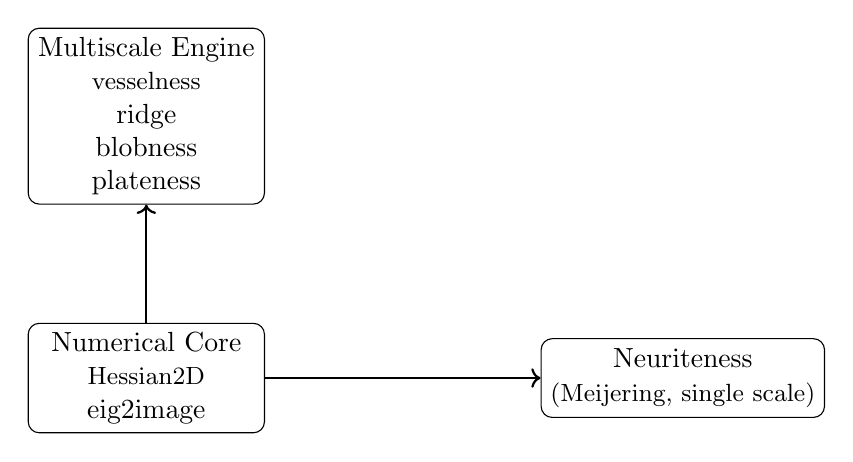
\begin{tikzpicture}[
			box/.style={draw, rounded corners, align=center, minimum width=3cm, minimum height=1cm},
			arrow/.style={->, thick}
			]
			
			% Core
			\node[box] (core) {Numerical Core\\\small Hessian2D\\eig2image};
			
			% Engine
			\node[box, above=1.5cm of core] (engine) {Multiscale Engine\\\small vesselness\\ridge\\blobness\\plateness};
			
			% Neuriteness
			\node[box, right=3.5cm of core] (neurite) {Neuriteness\\\small (Meijering, single scale)};
			
			% Arrows
			\draw[arrow] (core) -- (engine);
			\draw[arrow] (core) -- (neurite);
			
		\end{tikzpicture}
		\caption{Software architecture showing shared numerical primitives and separation between multiscale Hessian detectors and single-scale neuriteness.}
	\end{figure}
	
	
	\subsection{Core Functions}
	
	\begin{description}
		\item[\texttt{Hessian2D.m}] Computes second-order Gaussian derivatives.
		\item[\texttt{eig2image.m}] Eigenvalues and eigenvectors of the Hessian.
	\end{description}
	
	\subsection{Multiscale Engine}
	
	\texttt{hessian2DFilters.m} implements vesselness, ridge, blob, and plate filters using a max-over-scales strategy.
	
	\subsection{Neuriteness}
	
	\texttt{neuriteness2D.m} implements the Meijering neuriteness filter exactly as described in the literature.
	
	% -----------------------------------------------------------------------------
	\section{Test Suite}
	
	The accompanying test suite is layered to match the architecture:
	\begin{itemize}
		\item numerical invariants (Hessian, eigenvalues),
		\item detector semantics (vesselness),
		\item shape invariants (neuriteness).
	\end{itemize}
	
	Each test enforces a documented mathematical or algorithmic guarantee; no test asserts behaviour not promised by the underlying theory.
	
	% -----------------------------------------------------------------------------
% -----------------------------------------------------------------------------
\section{Synthetic Benchmark Phantom}

To illustrate the differing assumptions and response characteristics of
multiscale Hessian-based detectors and single-scale neuriteness, we employ
a synthetic benchmark image containing a mixture of geometric primitives:

\begin{itemize}
	\item thin and thick curvilinear structures,
	\item intersections at multiple orientations,
	\item isotropic blob-like structures,
	\item plate-like regions with low curvature anisotropy.
\end{itemize}

This composite phantom intentionally violates the assumptions of any single
structure model, making it suitable for qualitative comparison.
\pagebreak

\begin{figure*}[ht]
	\centering
	\includegraphics[width =1\linewidth
	]{figures/complex_composite.pdf}
	\vspace{-9.5 cm}
	\caption{Composite comparison of Hessian-based filters on the synthetic benchmark phantom.
		(a) Input image.
		(b) Vesselness.
		(c) Blobness.
		(d) Plateness.
		(e) Neuriteness.}
\end{figure*}

\newpage
	\section{Demos and Figure Generation}
	
	\subsection{Demo Script}
	
	The following MATLAB script generates figures used in this manual.
	
	\begin{lstlisting}[language=Matlab,caption={Demo script to generate figures for the manual}]
		% demo_generate_figures.m
		Iline = generateTestLineImage(256,30,3);
		Iblob = generateTestBlobImage(256,10);
		
		[V,~,D] = hessian2DFilters(Iline, ...
		'FilterType','vesselness', ...
		'Sigmas',1:4, ...
		'Parameters',struct('beta',0.5,'c',15));
		
		[N,DN] = neuriteness2D(Iline,2);
		
		figure; imagesc(Iline); axis image off; colormap gray;
		title('Input image');
		
		figure; imagesc(V); axis image off; colormap hot;
		title('Vesselness response');
		
		figure; imagesc(N); axis image off; colormap hot;
		title('Neuriteness response');
	\end{lstlisting}
	
	Figures produced by this script can be saved and included as PDF files in the \texttt{figures/} directory for use in this document.
	
	In addition to simple line and blob examples, a more complex synthetic
	benchmark phantom is generated to highlight the complementary behavior
	of multiscale vesselness and single-scale neuriteness filters.
	
	% -----------------------------------------------------------------------------
	\section{Repository Layout and Build Instructions}
	
	\subsection{Folder Structure}
	
\begin{verbatim}
	hessian-neuriteness/
	|-- core/
	|   |-- Hessian2D.m
	|   |-- eig2image.m
	|   `-- hessianEigen2D.m
	|
	|-- engine/
	|-- neuriteness/
	|-- demos/
	|-- tests/
	`-- manual/
\end{verbatim}

	
	\subsection{Building the Manual}
	
	\begin{verbatim}
		cd manual
		pdflatex manual.tex
		bibtex manual
		pdflatex manual.tex
		pdflatex manual.tex
	\end{verbatim}
	
	\section{Test Suite}
	
	The test suite mirrors the architecture of the codebase:
	
	\begin{itemize}
		\item \textbf{Core tests}: numerical invariants of Hessian derivatives and eigenvalues.
		\item \textbf{Engine tests}: detection semantics for multiscale Hessian filters.
		\item \textbf{Neuriteness tests}: shape continuity and orientation invariants.
	\end{itemize}
	
	No test asserts behavior not guaranteed by the underlying theory.
	
\begin{thebibliography}{9}
	
	\bibitem[Frangi et~al.(1998)]{Frangi1998}
	A.~F. Frangi, W.~J. Niessen, K.~L. Vincken, and M.~A. Viergever.
	\newblock Multiscale vessel enhancement filtering.
	\newblock \emph{Medical Image Computing and Computer-Assisted Intervention}, 1998.
	
	\bibitem[Meijering et~al.(2004)]{Meijering2004}
	E.~Meijering, M.~Jacob, J.-C. Sarria, P.~Steiner, H.~Hirling, and M.~Unser.
	\newblock Design and validation of a tool for neurite tracing and analysis in fluorescence microscopy images.
	\newblock \emph{Cytometry Part A}, 58A:167--176, 2004.
	
	\bibitem[Lindeberg(1998)]{Lindeberg1998}
	T.~Lindeberg.
	\newblock Feature detection with automatic scale selection.
	\newblock \emph{International Journal of Computer Vision}, 30(2):79--116, 1998.
	
\end{thebibliography}

\end{document}
